\documentclass[11pt,a4paper]{article}
\usepackage[T1]{fontenc}
\usepackage{lmodern}
\usepackage[top=0.78in, bottom=0.78in, left=0.84in, right=0.84in]{geometry}
\usepackage{amsmath,amssymb}
\usepackage{graphicx}
\usepackage{tikz}
\usetikzlibrary{arrows.meta,positioning,calc}
\usepackage{tcolorbox}
\usepackage{hyperref}
\usepackage{booktabs}
\usepackage{caption}

\hypersetup{colorlinks=true, linkcolor=blue!70!black, urlcolor=blue!70!black}

\newtcolorbox{learningobj}{
    colback=blue!3!white, colframe=blue!60!black,
    fonttitle=\bfseries\sffamily, title={$\blacktriangleright$ LEARNING OBJECTIVE},
    arc=2mm, boxrule=1pt, left=4mm, right=4mm, top=2mm, bottom=2mm
}
\newtcolorbox{physicalinsight}{
    colback=yellow!6!white, colframe=orange!75!black,
    fonttitle=\bfseries\sffamily, title={$\blacktriangleright$ PHYSICAL INSIGHT},
    arc=2mm, boxrule=1pt, left=4mm, right=4mm, top=2mm, bottom=2mm
}
\newtcolorbox{equationcard}{
    colback=green!3!white, colframe=green!45!black,
    fonttitle=\bfseries\sffamily, title={Equation card},
    arc=2mm, boxrule=1pt, left=4mm, right=4mm, top=2mm, bottom=2mm
}
\newtcolorbox{misconceptionbox}[1]{
    colback=red!2!white, colframe=red!70!black,
    fonttitle=\bfseries\sffamily, title={$\triangle$ TRAP: #1},
    arc=2mm, boxrule=0.8pt, left=3.5mm, right=3.5mm, top=1.5mm, bottom=1.5mm
}

\renewcommand{\thefigure}{1.1.5\alph{figure}}
\captionsetup{font=small, skip=4pt}

\begin{document}

\section*{1.1.5 The Sample Is Not Air Pressure Yet}

\begin{learningobj}
Section 1.2 will take a finite packet of samples and turn it into a spectrum. This section is about the word that arrives before that packet exists. A digital microphone spends a fixed number of bit clocks emitting exact zeros, and the high-pass already inside the microphone sits far below the pitch of a voice. We derive the length of the mute at $16\text{ kHz}$, add one biquad high-pass at $60\text{ Hz}$, and hold the ring buffer closed until both the mute and the filter's own startup have passed.
\end{learningobj}

Section 1.1 closed on a dilemma: an edge processor has to cut an unending pressure wave into finite packets, and it may not wait for a batch. Section 1.2 answers with a ring buffer, a window, and a transform. Both of those sections are right about the packet. They start one step late. The number that leaves an I\textsuperscript{2}S microphone is a 24-bit word. It becomes a sample of air pressure only after two gates have opened.

The frontend this book builds listens at $f_s = 16\text{ kHz}$. One sample period is $62.5\,\mu\text{s}$. The buffer that Section 1.2 will close holds 400 samples, and it steps forward by 160 samples, which is $10\text{ ms}$. The lowest pitch that buffer is asked to keep is $85\text{ Hz}$. The first vowel resonance sits near $300\text{ Hz}$. Anything this section removes has to be gone before those 400 samples are sealed, because the transform never sees the raw word. It sees the sealed frame.

\subsection*{A quarter of a second of exact zeros}

The microphone in front of this pipeline is the INMP441, a bottom-port MEMS microphone with a 24-bit I\textsuperscript{2}S word. Its datasheet states a startup rule in one sentence: the microphone has zero output for the first $2^{18}$ SCK cycles after power-up. The same page gives the check on that count. At an SCK of $3.072\text{ MHz}$ the mute lasts $85\text{ ms}$.

$2^{18}$ is $262{,}144$. Divided by $3.072\text{ MHz}$ that is $85.333\text{ ms}$. The datasheet's $85\text{ ms}$ is that quotient, rounded. The count is doing the work. The milliseconds are the count at one particular clock.

The same datasheet fixes how many bit clocks make one output frame. The data word is 24 bits, and the part still demands 64 SCK cycles in each stereo frame:
\begin{equation*}
f_{\mathrm{SCK}} = 64 \times f_{\mathrm{WS}}
\end{equation*}
$f_{\mathrm{WS}}$ is the rate of the word-select line, which is the sample rate of the stream. At the $16\text{ kHz}$ of this book the bit clock is $64 \times 16{,}000 = 1{,}024{,}000\text{ Hz}$.

\begin{equationcard}
\textbf{The formula.}
\[
T_{\mathrm{mute}} = \frac{2^{18}}{64\, f_s}
\]
\textbf{The variables.}
\begin{itemize}\setlength{\itemsep}{1pt}
    \item $T_{\mathrm{mute}}$ --- time from the first bit clock to the first nonzero output word, in seconds.
    \item $2^{18}$ --- the startup count in the INMP441 datasheet, in SCK cycles. The output word is zero for every cycle of that count.
    \item $64$ --- SCK cycles in one stereo frame, the datasheet rule $f_{\mathrm{SCK}} = 64 \times f_{\mathrm{WS}}$.
    \item $f_s$ --- the sample rate, in Hz. Here it is $16{,}000$, and it is also $f_{\mathrm{WS}}$.
\end{itemize}
\textbf{What it means.} The mute is a count of bit clocks, so a slower sample rate makes it last longer. The datasheet's $85\text{ ms}$ belongs to a $3.072\text{ MHz}$ bit clock. This book's bit clock is $1.024\text{ MHz}$, and the same count lasts longer by that ratio.

\textbf{What it costs.} A counter and a write-enable. While the count runs, the ring buffer's write pointer does not move. No multiply is involved. The cost is paid once, at power-up.

\textbf{What it does not say.} The formula is the INMP441's mute at a 64-clock frame. A different microphone has a different count. It also says nothing about a pause between utterances. After the first nonzero word, the part is in normal operation and this timer has finished.
\end{equationcard}

The lab evaluates the formula at $16\text{ kHz}$:
\[
T_{\mathrm{mute}} = \frac{262{,}144}{1{,}024{,}000} = 0.256\text{ s}
\]
That is $4{,}096$ samples. A hop of 160 samples divides it into $25.6$ hops. The mute therefore covers 25 whole hops and 96 samples of the next one. A buffer that started at the first clock would seal a frame across that boundary: 96 zeros, then the first real words, which a transform reads as a step. Discarding the $4{,}096$ zero words means that frame is never built. The write pointer starts at the first nonzero word.

\begin{physicalinsight}
The $256\text{ ms}$ is a boot hold, paid once per power-up. The $10\text{ ms}$ deadline from Section 1.1 starts when the write pointer is released. Counting $256\text{ ms}$ inside the latency of each spoken word counts this timer once per utterance.
\end{physicalinsight}

\subsection*{The high-pass inside the microphone is a different filter}

A natural next belief is that the part has already cleaned the low end, so the processor can start Section 1.2 at once. The datasheet does contain a high-pass. Read at $16\text{ kHz}$, it sits far below a voice.

Table 7 gives the digital high-pass at a nominal $48\text{ kHz}$: $-3\text{ dB}$ at $3.7\text{ Hz}$, $-0.5\text{ dB}$ at $10.4\text{ Hz}$, and $-0.1\text{ dB}$ at $21.6\text{ Hz}$. The same paragraph says the cutoff scales with the sampling rate. Scaling by $16/48$ moves those three points to $1.2333\text{ Hz}$, $3.4667\text{ Hz}$, and $7.2000\text{ Hz}$. By about $7\text{ Hz}$ the microphone's own digital filter has come back to a tenth of a decibel. It removes a true drift inside the part. It is finished long before the lowest pitch.

There is a second, mechanical corner. The MEMS element itself is $-3\text{ dB}$ at $60\text{ Hz}$, and the datasheet says the digital filter sits on top of that acoustic corner. A $-3\text{ dB}$ point is a gentle shoulder. Between roughly $7\text{ Hz}$ and the $85\text{ Hz}$ pitch, the word still carries rumble, handling, and whatever offset the $1.2333\text{ Hz}$ filter has not yet forgotten.

\subsection*{One biquad, placed under the pitch}

The stage this section adds is a single biquad high-pass, the form in Robert Bristow-Johnson's Audio EQ Cookbook. The cutoff is $60\text{ Hz}$, on the microphone's acoustic corner and under the $85\text{ Hz}$ pitch. The cookbook still requires a quality factor. This section uses the Butterworth value $Q = 1/\sqrt{2}$, so the passband does not peak. A progress note from 20 October 2026 ran a cookbook high-pass near $60\text{ Hz}$ in floating point on an ESP32, ahead of any spectrum. That note does not fix $Q$. The value here is this section's choice, made so the arithmetic has one answer.

\begin{equationcard}
\textbf{The formula.}
\begin{align*}
\omega_0 &= 2\pi f_c / f_s \\
\alpha &= \sin\omega_0 / (2Q) \\
b_0 &= (1+\cos\omega_0)/2, \quad b_1 = -(1+\cos\omega_0), \quad b_2 = (1+\cos\omega_0)/2 \\
a_0 &= 1+\alpha, \quad a_1 = -2\cos\omega_0, \quad a_2 = 1-\alpha
\end{align*}
After division by $a_0$, the recurrence that runs on each sample is
\begin{align*}
y[n] &= b_0\, x[n] + z_1 \\
z_1 &\leftarrow b_1\, x[n] - a_1\, y[n] + z_2 \\
z_2 &\leftarrow b_2\, x[n] - a_2\, y[n]
\end{align*}
\textbf{The variables.}
\begin{itemize}\setlength{\itemsep}{1pt}
    \item $x[n]$ --- the input word at sample $n$, as a fraction of full scale.
    \item $y[n]$ --- the output sample at the same index.
    \item $f_c$ --- the cutoff, in Hz. Here $60$.
    \item $f_s$ --- the sample rate, in Hz. Here $16{,}000$.
    \item $Q$ --- the quality factor, dimensionless. Here $1/\sqrt{2}$, which the lab prints as $0.707107$.
    \item $\omega_0$ --- the cutoff in radians per sample.
    \item $\alpha$ --- the cookbook's intermediate width term, dimensionless.
    \item $b_0, b_1, b_2, a_1, a_2$ --- the five coefficients after $a_0$ has been divided out.
    \item $z_1, z_2$ --- the two stored delays. Both start at $0$ when the filter has never seen a sample.
\end{itemize}
\textbf{What it means.} The steady-state gain at $0\text{ Hz}$ is zero, because the three $b$ coefficients sum to zero. That zero is a property of the settled filter. On the first sample the delays are still empty, so $y[0] = b_0\, x[0]$. The lab's $b_0$ is $0.983477$. A unit step therefore comes out almost whole on the first sample, and the cancellation arrives only as $z_1$ and $z_2$ fill.

\textbf{What it costs.} Five multiplies and four adds per sample, and two stored words. At $16\text{ kHz}$ that is $80{,}000$ multiplies each second. The sample period is $62.5\,\mu\text{s}$, and the loop has that long to finish, because $y[n]$ depends on the delays left by the previous sample. This section does not turn those five multiplies into a DSP-slice count. The placement is the price that matters: the loop runs on the raw word, before a frame of 400 samples exists.

\textbf{What it does not say.} It does not remove a noise that shares the band with the vowel. It does not stand in for the window in Section 1.2. A larger $Q$ would peak above the cutoff and ring for longer. And $b_0 = 0.983477$ on the first sample of a unit step means the filter shortens the thump. The thump is still present on sample 0.
\end{equationcard}

The lab normalizes the cookbook at these two frequencies and prints:

\begin{center}
\begin{tabular}{lr}
\toprule
Coefficient & Value \\
\midrule
$b_0$ & $0.983477$ \\
$b_1$ & $-1.966954$ \\
$b_2$ & $0.983477$ \\
$a_1$ & $-1.966681$ \\
$a_2$ & $0.967227$ \\
\bottomrule
\end{tabular}
\end{center}

The gain at $0\text{ Hz}$ prints as $0$. The magnitude at the probes a voice designer actually argues about:

\begin{center}
\begin{tabular}{lrr}
\toprule
Frequency & Role & Gain \\
\midrule
$20\text{ Hz}$ & rumble, under the pitch & $-19.14\text{ dB}$ \\
$40\text{ Hz}$ & still under the pitch & $-7.83\text{ dB}$ \\
$60\text{ Hz}$ & the cutoff & $-3.01\text{ dB}$ \\
$80\text{ Hz}$ & just under the lowest pitch & $-1.19\text{ dB}$ \\
$85\text{ Hz}$ & the lowest pitch Section 1.2 keeps & $-0.96\text{ dB}$ \\
$300\text{ Hz}$ & the first vowel resonance & $-0.01\text{ dB}$ \\
\bottomrule
\end{tabular}
\end{center}

The deep cut is at $20\text{ Hz}$ and $40\text{ Hz}$. At $80\text{ Hz}$ the response is already on the shoulder, $1.19\text{ dB}$ down. This filter is $-3.01\text{ dB}$ at its $60\text{ Hz}$ cutoff, and the $85\text{ Hz}$ pitch loses $0.96\text{ dB}$.

\begin{figure}[ht]
\centering
% Block diagram for section 1.1.5. The ring buffer is where section 1.2 begins.
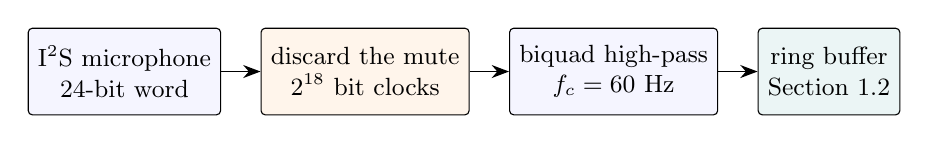
\begin{tikzpicture}[
    font=\small,
    node distance=5mm,
    box/.style={draw, rounded corners=1.5pt, align=center, minimum height=11mm, inner sep=3.5pt, fill=blue!4},
    gate/.style={draw, rounded corners=1.5pt, align=center, minimum height=11mm, inner sep=3.5pt, fill=orange!8},
    arr/.style={-{Stealth[length=2.2mm]}, semithick}
]
    \node[box] (mic) {I\textsuperscript{2}S microphone\\24-bit word};
    \node[gate, right=of mic] (mute) {discard the mute\\$2^{18}$ bit clocks};
    \node[box, right=of mute] (hpf) {biquad high-pass\\$f_c = 60\text{ Hz}$};
    \node[box, right=of hpf, fill=teal!8] (ring) {ring buffer\\Section 1.2};
    \draw[arr] (mic) -- (mute);
    \draw[arr] (mute) -- (hpf);
    \draw[arr] (hpf) -- (ring);
\end{tikzpicture}

\caption{Where the two gates sit. The I\textsuperscript{2}S word is discarded for the mute, then passed through the biquad, and only then written into the ring buffer that Section 1.2 reads. The spectral stages see neither the zero run nor the raw offset.}
\end{figure}

\begin{figure}[ht]
\centering
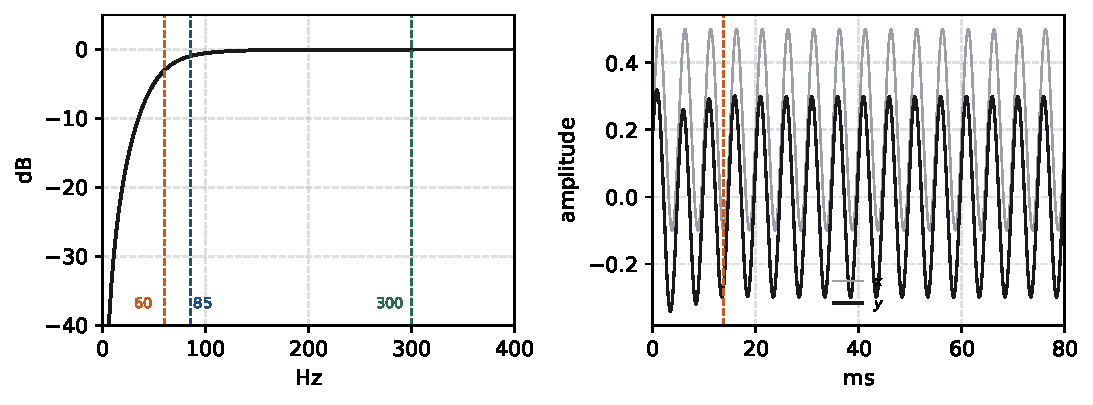
\includegraphics[width=\textwidth]{fig_1_1_5_response.pdf}
\caption{Left, the calculated magnitude from $5\text{ Hz}$ to $400\text{ Hz}$. The dashed lines mark $60\text{ Hz}$, $85\text{ Hz}$, and $300\text{ Hz}$. Right, a constructed input $x = 0.2 + 0.3\sin(2\pi\cdot 200\, t)$ and the filter output $y$. The dashed line in the time panel is the settling index from the lab. This panel is a calculation on a constructed wave.}
\end{figure}

On a unit step, with both delays starting at rest, the lab holds the output under $1\%$ of the step for one full hop of 160 samples. The first sample of that quiet run is sample $219$, which is $13.688\text{ ms}$. Those 219 outputs are the filter waking up. They stay out of the ring buffer. A spoken word is a different shape from a unit step, so $219$ is the step's number, the plain offset this section uses as its test.

The same lab drives a constructed $80\text{ ms}$ wave, an offset of $0.2$ plus a $200\text{ Hz}$ tone of amplitude $0.3$. The mean of the input is $0.2000$. The mean of the output after sample $219$ is $-0.0020$. The $200\text{ Hz}$ component, measured by correlation against a sinusoid on that same tail, moves from $0.2087$ to $0.2096$. The offset collapses. The tone in the passband stays.

While the microphone is still inside its mute, the input is exact zero and both delays stay at rest. The $13.688\text{ ms}$ therefore begins at the first nonzero word, after the $256\text{ ms}$, and the two holds follow one another. The write pointer is released when the step test says the state has entered the $1\%$ band. From the first bit clock to that release is $4{,}096 + 219 = 4{,}315$ samples.

\subsection*{What breaks if this stage is left out}

Feed the zero run to the ring buffer and the first frames are a digital mute. The transform of a mute is a mute, and the frame that straddles the first real word is a step, which spreads across the bins Section 1.2 is about to build. Leave the offset in a sealed frame and a constant, tapered by the window of Section 1.2, becomes that window's own spectrum sitting on the lowest bins. The window was built to soften a boundary. A constant that runs through the whole frame needs the biquad instead.

The October 2026 bench reported a change in the silence after this kind of filter. That log is absent from this repository. The decibel change from the bench is outside the results of this section. Figure 1.1.5b is the filter's calculated response, and the tables above are the lab that drew it.

\subsection*{Three traps}

\begin{misconceptionbox}{The datasheet high-pass already did this job}
The part does contain a digital high-pass. At $16\text{ kHz}$ its $-3\text{ dB}$ point sits at $1.2333\text{ Hz}$. The biquad in this section sits at $60\text{ Hz}$. They are stacked. One does not stand in for the other.
\end{misconceptionbox}

\begin{misconceptionbox}{The boot hold belongs inside the hop budget}
The $10\text{ ms}$ deadline is the time between sealed frames once the pointer is moving. The mute counter runs before the pointer moves. Adding $256\text{ ms}$ to every word's latency counts a power-up timer as a per-frame pipeline stage.
\end{misconceptionbox}

\begin{misconceptionbox}{A cutoff near $300\text{ Hz}$ would clean the feature}
A cutoff near the first vowel resonance would eat the resonance Section 1.2 exists to measure. The $60\text{ Hz}$ choice leaves $300\text{ Hz}$ at $-0.01\text{ dB}$ and the $85\text{ Hz}$ pitch at $-0.96\text{ dB}$. The offset is gone, and the pitch is still in the frame.
\end{misconceptionbox}

\subsection*{The unresolved dilemma: the noise that shares the vowel}

The mute is gone and the offset is dying. A noise that lives between $300\text{ Hz}$ and the top of the speech band is still inside every sample the ring buffer will seal. The biquad has no opinion about it. Section 1.2 can now start, because the word it receives is a slice of the pressure wave. The noise that shares the vowel's band is still in that slice.

\subsection*{Where the numbers come from}

\begin{center}
\small
\begin{tabular}{p{0.38\textwidth} p{0.54\textwidth}}
\toprule
Source & What it says \\
\midrule
INMP441 datasheet, DS-INMP441-00, revision 1.1, Startup and Data Word Length &
Zero output for the first $2^{18}$ SCK cycles, with the parenthetical $85\text{ ms}$ at an SCK of $3.072\text{ MHz}$. There are 64 SCK cycles in each stereo frame, written $f_{\mathrm{SCK}} = 64 \times f_{\mathrm{WS}}$. \\
\addlinespace
The same datasheet, Table 7 and the sentence under it, plus Table 1 &
The digital high-pass at a nominal $48\text{ kHz}$ is $-3\text{ dB}$ at $3.7\text{ Hz}$, $-0.5\text{ dB}$ at $10.4\text{ Hz}$, $-0.1\text{ dB}$ at $21.6\text{ Hz}$, and the cutoff scales with sample rate. The MEMS element is $-3\text{ dB}$ at $60\text{ Hz}$, in addition to that digital filter. \\
\addlinespace
Robert Bristow-Johnson, Cookbook formulae for audio EQ biquad filter coefficients &
The high-pass coefficient formulas used above, before the division by $a_0$. \\
\addlinespace
\texttt{results/lab115/20261020T175727Z/} \texttt{stdout.log} and \texttt{result.json} &
Every derived figure in this section: $85.333\text{ ms}$, $0.256\text{ s}$, $4{,}096$ samples, $25.6$ hops, the scaled trio $1.2333$, $3.4667$, $7.2000\text{ Hz}$, the five coefficients, the six probe gains, sample $219$ at $13.688\text{ ms}$, and the constructed means $0.2000$ and $-0.0020$ with tone components $0.2087$ and $0.2096$. Both files are listed in \texttt{results/SHA256SUMS}. The curves are drawn by \texttt{lab\_1\_1\_5.py}. \\
\bottomrule
\end{tabular}
\end{center}

\end{document}
